\documentclass[12pt]{report}
\usepackage[utf8]{inputenc}
\usepackage[french]{babel}
\usepackage[T1]{fontenc}
\usepackage{amsmath}
\usepackage{amsfonts}
\usepackage{amssymb}
\usepackage{graphicx}
\usepackage{titlesec}
\usepackage{caption}
\usepackage{titling}
\usepackage{booktabs}
\usepackage{enumitem}
\usepackage{eurosym}
\usepackage{epigraph}
\usepackage{hyperref}
\usepackage{fontspec}
\usepackage{ragged2e}
\usepackage{parskip}
\usepackage{wrapfig}
\usepackage{calc}
\usepackage{float}

\graphicspath{ {../../static/} {img/} }
\setlength{\droptitle}{-10em}
\titleformat{\chapter}[hang]{\normalfont\huge\bfseries}{\thechapter. }{0em}{}

\begin{document}

\title{
	{\vspace{3em}\protect\centering\protect
\includegraphics[width=0.9\textwidth]{pacification_vector.pdf}}\\
	{\vspace{4em}\Huge Rapport de soutenance}\\
	{\large Brainless Devs}
}
\author{
	Thibault Allançon\\
	Valérian Fayt
	\and
	Antoine Gonzalez\\
	Cédric Parpet}
\date{
	{\vfill\protect\centering\protect
\includegraphics{brainless_devs.pdf}}\\
	Dossier Projet Informatique\\
	Info-Sup EPITA\\
	Mars 2018
}

\maketitle
\tableofcontents

\chapter{Introduction}

Cette première phase de développement de \textit{Pacification} aura été assez riche d'expérience. En effet, il a fallu partir de rien et poser les fondations de notre jeu. Cela aura été une phase de découverte de notre environnement de travail, et nous avons dû nous heurter à la réalité et adapter notre plan d'origine, en procédant à une légère réorganisation de la répartition des tâches.

Cette période aura été une période d'expérimentation pour notre partie réseau, de réflexion pour notre partie gameplay, et de préparation pour notre partie graphique. Toutefois, nos objectifs ont étés atteints. La map et le réseau sont fonctionnels, nous avons nos premiers assets qui pourront ensuite être réutilisés afin de gagner du temps. Pour finir, l'organisation du gameplay ainsi que des éléments du jeu est claire.

Cette première partie du développement de ce projet a été une expérience personnelle instructive pour chacun. De manière générale, les engagements vis-à-vis du jeu sont tenus, ainsi que le planning mis en place dans le cahier des charges.

Nous allons ici détailler l'état d'avancement de notre projet, ainsi que nos plans jusqu'à la deuxième soutenance.

\begin{figure}
    \centering
    
\includegraphics[width=0.6\textwidth]{project_mood_S1}
    \caption*{\textit{Calvin and Hobbes}, Bill Watterson}
\end{figure}

\chapter{Cahier des charges}

Le cahier des charges nous semble toujours satisfaisant, nos objectifs sont atteignables, et il n'y a selon nous rien à ajouter au jeu qui n'ait pas été mentionné dans le cahier des charges. La répartition des tâches est convenable, bien que certains changements auront lieu pour la seconde période : Antoine et Valérian deviendront suppléants UI pour établir l'interface anglais/français dans le jeu, et assister Cédric qui sera très occupé par les assets.

\begin{center}
    \begin{tabular}{@{} l *4c @{}}
        \toprule
        \multicolumn{1}{c}{}    & \textbf{Thibault}  & \textbf{Antoine}  & \textbf{Cédric} & \textbf{Valérian} \\ 
        \midrule
        Map & R & S & & \\
        IA & R & & & \\
        Réseau & & S & S & R \\
        Graphisme & & & R & \\
        UI & & \underline{\textbf S} & R & \underline{\textbf S} \\
        Site web & & & & R \\
        Gameplay & S & R & & S\\
        \bottomrule
        \multicolumn{4}{l}{\footnotesize R = responsable, S = suppléant}\\
    \end{tabular}
\end{center}

Les assets faits à la main sont longs à réaliser, nous sommes donc plus proche de 40\% que de 50\% d'assets. Toutefois, les résultats sont visuellement très satisfaisants et l'investissement en temps en vaut la peine. De plus, la vitesse de production va s'accélérer pour les prochaines phases du projet car certains modèles serviront de bases pour ceux à venir.

 En ce qui concerne l'IA, les 30\% prévus étaient ambitieux sachant qu'il n'y a pas encore suffisamment d'éléments de gameplay implémenté. Nous avons donc établi le fonctionnement de cette dernière ainsi que ses caractéristiques principales qui permettront une implémentation rapide.

\chapter{Avancement}

\section{Map (Thibault)}

L’ensemble du jeu repose entièrement sur la carte, il était donc fondamental de s’y attaquer le plus tôt possible et d’implémenter rapidement le strict nécessaire pour développer le reste du jeu.

La particularité de la map étant qu’elle est constituée d’hexagone, il fallait donc correctement prendre cela en compte tant pour l’aspect graphique (rendu visuel, pavage) que l’aspect technique (nouveau système de coordonnées/déplacement, gérer correctement les relations de voisins).

\begin{figure}[H]
    \centering
    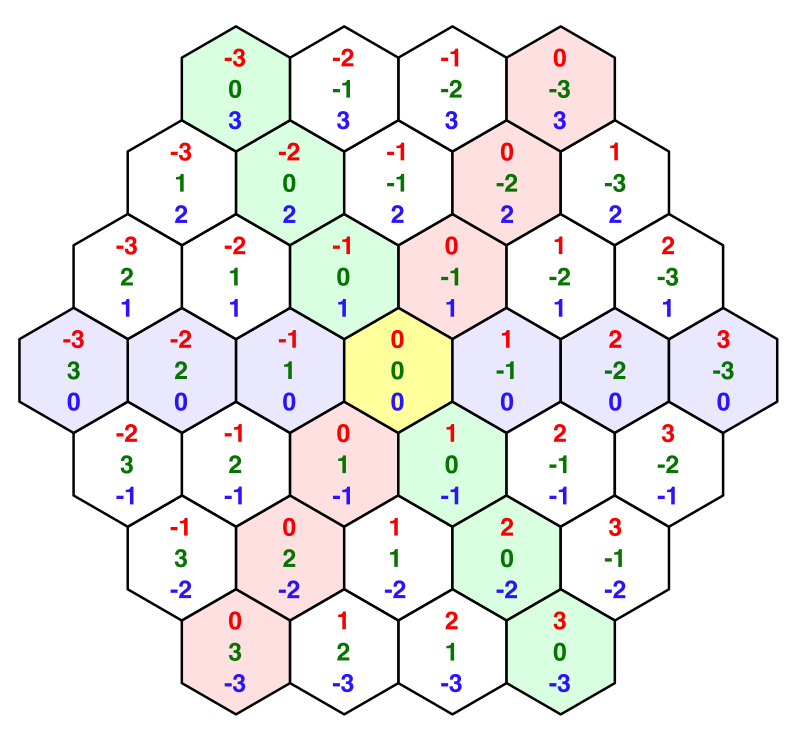
\includegraphics[width=0.5\textwidth]{cubic_coordinates}
    \caption{Système de coordonées et axes}
\end{figure}

De plus la carte est découpée en chunks afin de faciliter le rendu et avoir une meilleur fluidité sur des tailles de carte conséquente. En effet, utiliser un seul mesh pour toute une carte n’est clairement pas envisageable, surtout en anticipant le multijoueur, il faut donc découper cette dernière en chunks qui ont chacun leurs propres mesh. Lors d’une mise à jour de la map, il suffit alors de mettre à jour quelques chunks et non toute la carte (ce qui allège considérablement le rendu graphique).

Actuellement la carte présente différentes caractéristiques modifiables : des biomes pour les cases, possibilité de créer des montagnes d’une hauteur variable, création de routes pour relier des cases entre elles. Tout ceci a nécessité une manière d’intéragir et de se déplacer sur la carte en jeu (déplacement de la caméra, détection du clic et identification de la case sélectionnée, zoom).

Un premier pas vers le support complet des unités a été fait en créant le système de pathfinding pour se déplacer sur la carte (prenant en compte des aspects tel que l’élévation, les routes, etc.). Le C\# ne disposant pas d’une classe pour créer des tas, il a fallu commencer par l’implémentation d’une file à priorité afin de mettre en place l’algorithme A*. Ce dernier est une variante de l’algorithme de Dijkstra pour calculer le plus court chemin dans un graphe pondéré positivement, et se base sur une heuristique afin d’accélérer la recherche de ce chemin.

\begin{figure}[H]
    \centering
    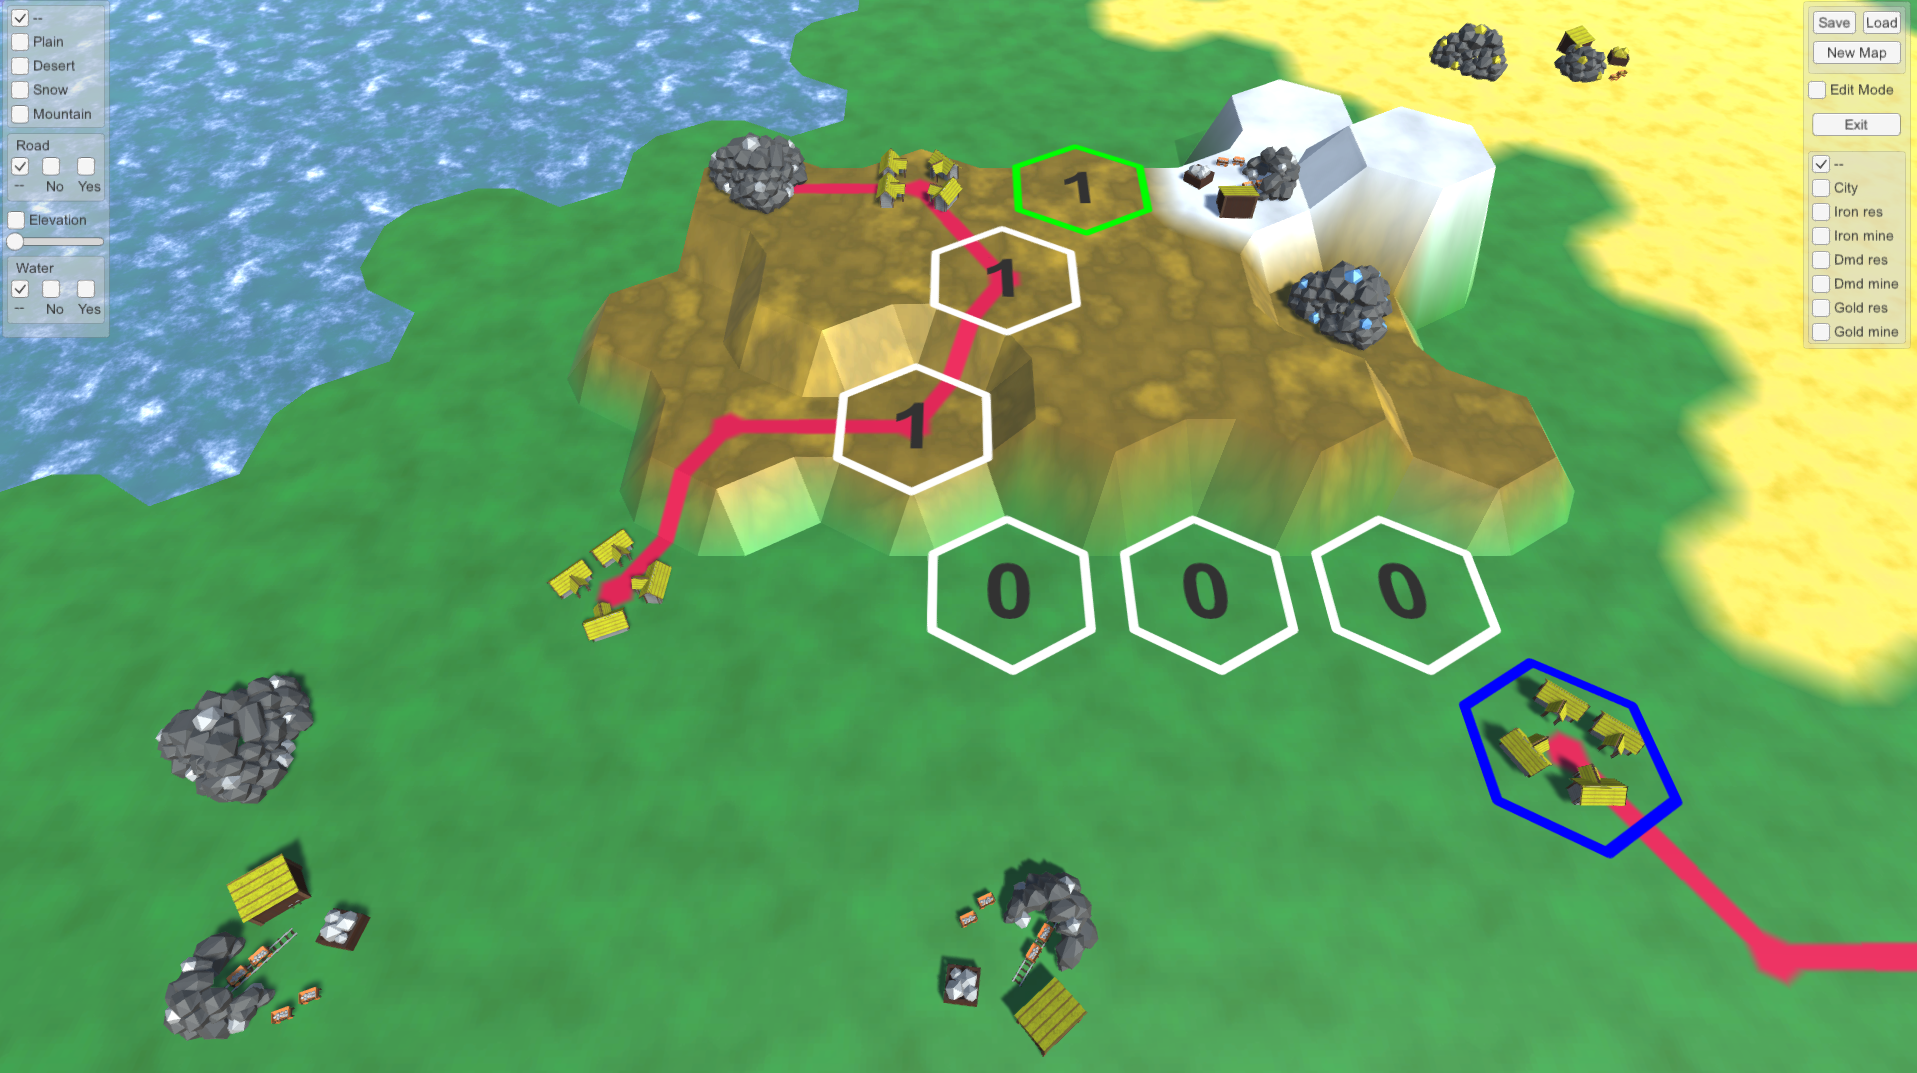
\includegraphics[width=0.8\textwidth]{map_features}
    \caption{Démonstration de la map}
\end{figure}

\newpage

Le système de sauvegarde et de chargement est aussi en place, il pourra permettre d’avoir un mode de création de ses propres cartes qu’on pourra ensuite sélectionner en solo ou en multi pour jouer dessus.

\begin{figure}[H]
    \centering
    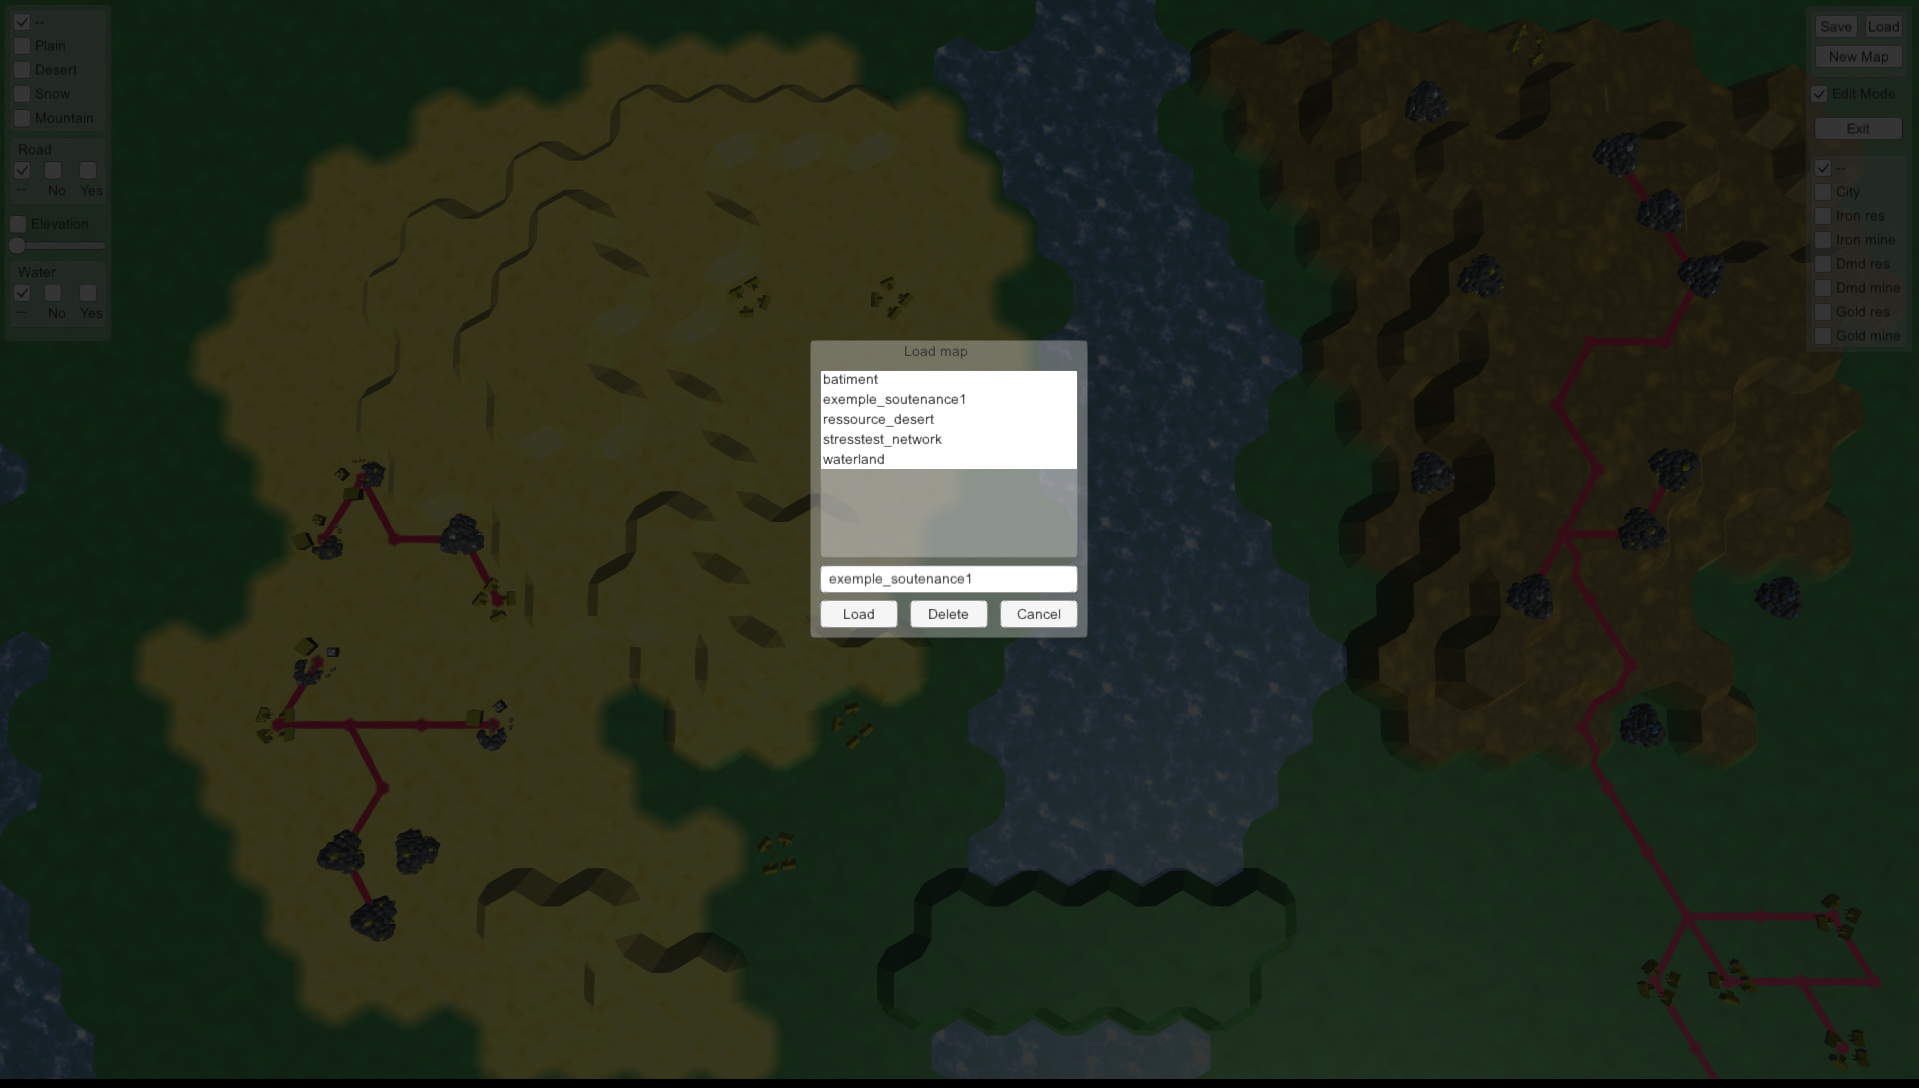
\includegraphics[width=0.8\textwidth]{map_save_load}
    \caption{Menu de sauvegarde/chargement}
\end{figure}

\section{Réseau et multijoueur (Valérian)}

L’implémentation du multijoueur étant essentielle pour le bon déroulement du jeu, il était prioritaire de le rendre fonctionnel. Contrairement à ce qui avait été envisagé, le multijoueur proposé basiquement par \textit{Unity} ne nous convenait pas, car ne nous permettait pas d’avoir un contrôle total sur cette partie. De plus, la perspective d’apprentissage était bien plus intéressante en passant par un codage par soi-même du multijoueur plutôt que d’utiliser une base déjà préfabriquée. Le serveur est donc démarré lorsqu’un joueur héberge la partie. Les clients quant à eux, sont activés automatiquement sur les ordinateurs des joueurs tentant de se connecter à un serveur pour rejoindre une partie. À noter que le joueur qui héberge possède lui aussi un client qui se connecte directement au serveur, au démarrage de celui-ci.

Lorsque le serveur est démarré, il commence à écouter dans l’attente de tentatives de connexions. Tant que le nombre de joueurs souhaité (de 2 à 8) n’est pas atteint, il continue d’attendre des connexion. Les clients se connectent à ce serveur à l’aide de l’adresse IP de l’hôte. À chaque tentative de connexion d’un client, le serveur lui demande de s’identifier, en lui envoyant en même temps la liste des identifiants des clients déjà connectés. Une fois l’identifiant obtenu, il est transmis aux autres clients. Si l’un des clients se déconnecte, le serveur transmet cette information aux clients encore en ligne. Ce processus permet à tous les joueurs de savoir à tout moment qui est connecté sur la partie.

\begin{figure}[H]
    \centering
    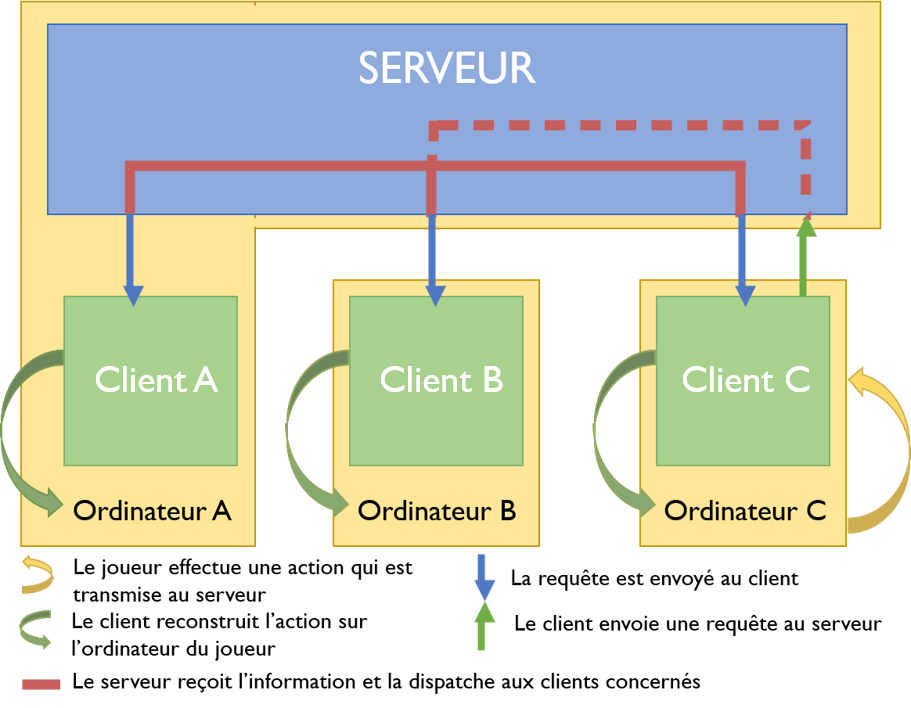
\includegraphics[width=0.8\textwidth]{multiplayer}
    \caption{Shéma fonctionnel du réseau}
\end{figure}

Quand le nombre de joueurs souhaité est atteint, le serveur n'accepte plus de connexion et transmet aux clients un message annonçant le début de la partie, ce qui a pour effet de démarrer celle-ci à la réception par les clients.

Pendant le jeu, les échanges sont effectués via un processus de sérialisation. Lorsqu’un joueur effectue une action, celle-ci est sérialisée sous forme de string puis envoyé au serveur qui se charge de dispatcher correctement le-dit message aux autres joueurs. À la réception d’un message, le client va reproduire l’action que ce message décrit. Le type d’action est défini par les quatres premiers caractères du message transmis : Le premier caractère indique le type de l’expéditeur (S pour le serveur, C pour un client) et les 3 suivant indiquent le type d’action.

\begin{center}
	\begin{tabular}{c|c}
		\toprule
		\textbf{Caractères}  & \textbf{Action}\\ 
		\midrule
		WHO & Demande d’identification \\
		IAM & Réponse d'identification \\
		CNN & Nouvelle connexion \\
		DEC & Déconnexion d’un client \\
		MAP & Transmission de la map \\
		END & Annonce de la fin d’un tour \\
		YGO & Autorisation de début de tour\\
		MOV & Mouvement d’unité effectué\\
		BDC & Construction d’un bâtiment\\
		BDM & Mise à jour d’un bâtiment\\
		EDI & Edition de la map\\
		MSG & Message global\\
		MSP & Message privé\\
		MSE & Erreur de destinataire du message\\
		\bottomrule
	\end{tabular}
\end{center}

\vspace{1em}

Ce système a ainsi permis la mise en place d’un suivi de l’état des clients (connecté / déconnecté) synchronisé sur tous les appareils, ainsi que la base d’un système de chat entre les joueurs (public et privé) mais aussi plus particulièrement la synchronisation des éditions de la map de jeu.

La latence qui pourrait survenir avec ce système n’est pas un problème dans le cas de ce projet, car il ne s’agit pas d’un jeu nécessitant une synchronisation en temps réel etant donné que les parties se déroulent en tour par tour.

Un exemple du processus pouvant être celui-ci :

\begin{itemize}[label=\textbullet]
	\item Le joueur \textit{player\_A} déplace une unité (numéroté 3) de la case $(5;3)$ vers la $(5;5)$
	\item Le client envoie le message\textit{ “CMOV|3\#5.3\#5.5”}
	\item Le serveur reçoit et renvoie aux clients\textit{ “SMOV|player\_A\#3\#5.3\#5.5”}
	\item Les clients reçoivent le message et le décryptent pour déplacer l’unité du \textit{playerF\_A}
\end{itemize}

\section{Gameplay (Antoine)}

Pour le moment, le gameplay était en phase de réflexion. Avant de commencer à implémenter les différents éléments du jeu, il était important pour nous de tout représenter visuellement de manière organisée afin de faire le maximum d’ajustements sans avoir à modifier de code (limitant ainsi les bugs et conflits).

L’élément le plus important est la hiérarchie des classes, qui permet de voir clairement quelle classe hérite de quelle autre classe, afin d’anticiper les héritages et d’éviter les attributs inutiles. Les autres liens entre les classes (contient/produit/énumérations de types) permettent d’anticiper des attributs et méthodes, en gardant le réseau et la map en tête pour chaque méthode. Enfin, l’organisation du diagramme permet de visualiser rapidement quelles classes sont à travailler en priorité, et d’identifier l’origine de certains bugs pouvant survenir au cours du développement (selon leurs dépendances).

Certains éléments ont commencé à être équilibrés (notamment les unités et les biomes), afin d’identifier un maximum d’attributs nécessaires à leur implémentation, et de paramètres à ajuster sur la map. Cet équilibrage semble pour le moment satisfaisant, mais sera probablement modifié pour la dernière soutenance, une fois que le jeu sera terminé et qu’il ne restera plus qu’à faire des ajustements minutieux suite à des tests en conditions réelles (les paramètres actuels n’étant issus que de calculs et de graphiques).

Nous avons par exemple différents tableaux qui donnent une idée précise de comment les unités interagissent entre elles, comment leurs statistiques évolueront au fil de la partie, et comment chaque biome affecte le jeu.

\begin{figure}[H]
    \centering
    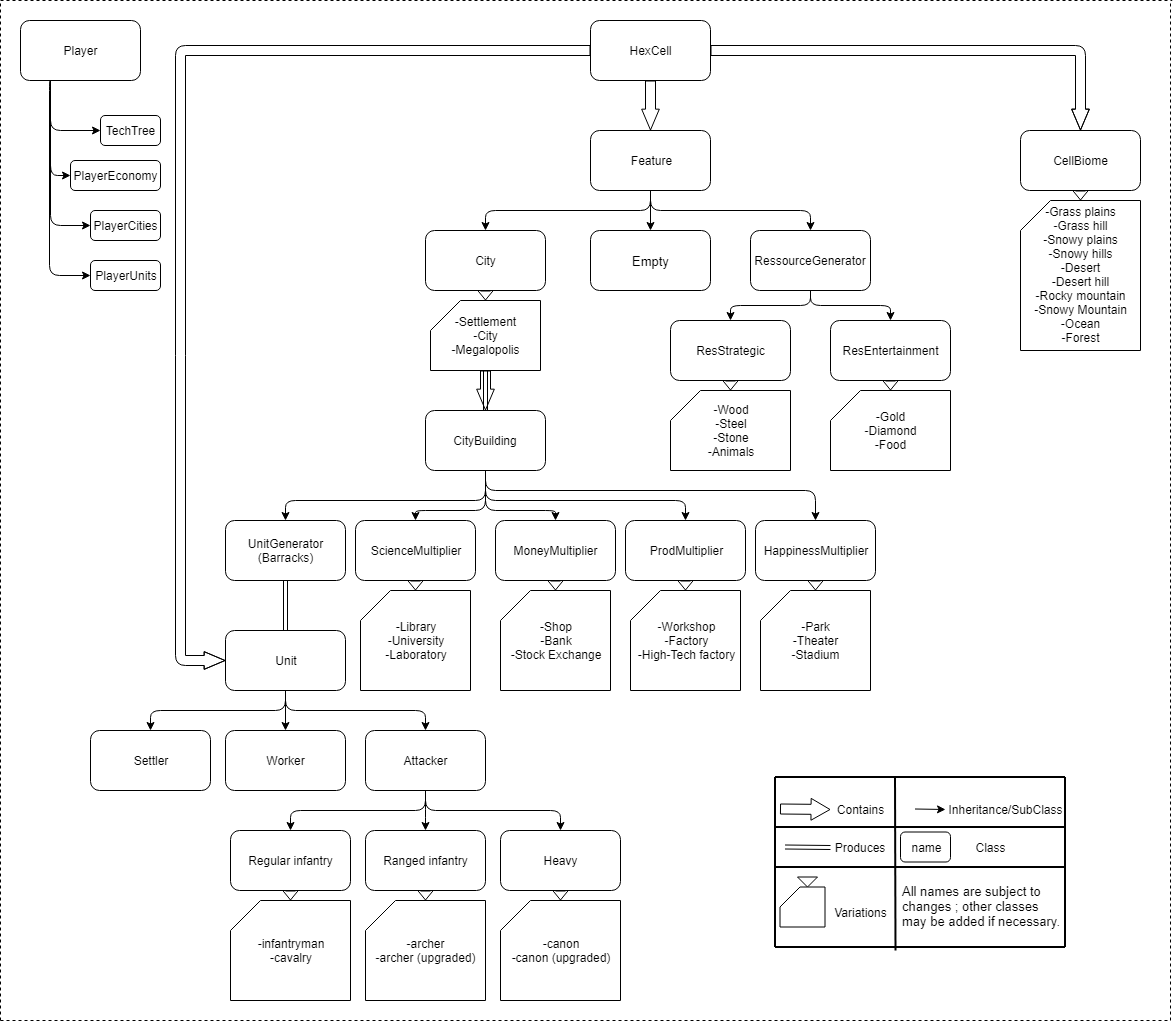
\includegraphics[width=1\textwidth]{class_hierarchy}
    \caption{Hiérarchie des classes}
\end{figure}

\begin{figure}[H]
    \centering
    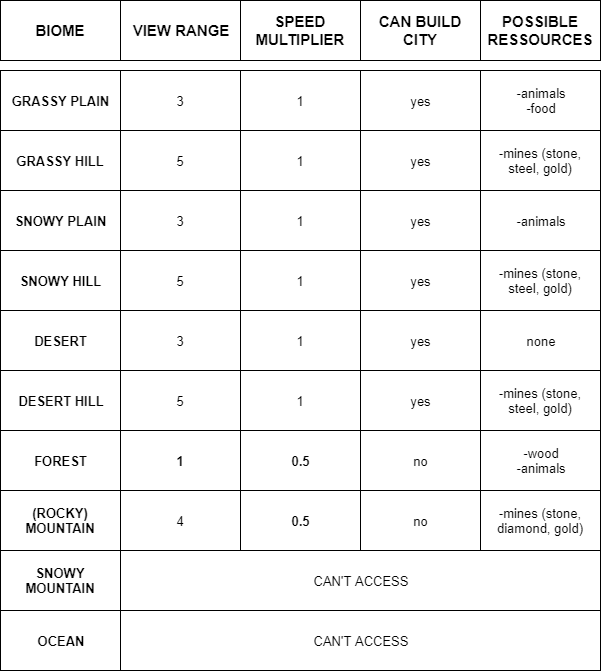
\includegraphics[width=0.9\textwidth]{biomes_effects}
    \caption{Effets des biomes}
\end{figure}
\begin{figure}[H]
    \centering
    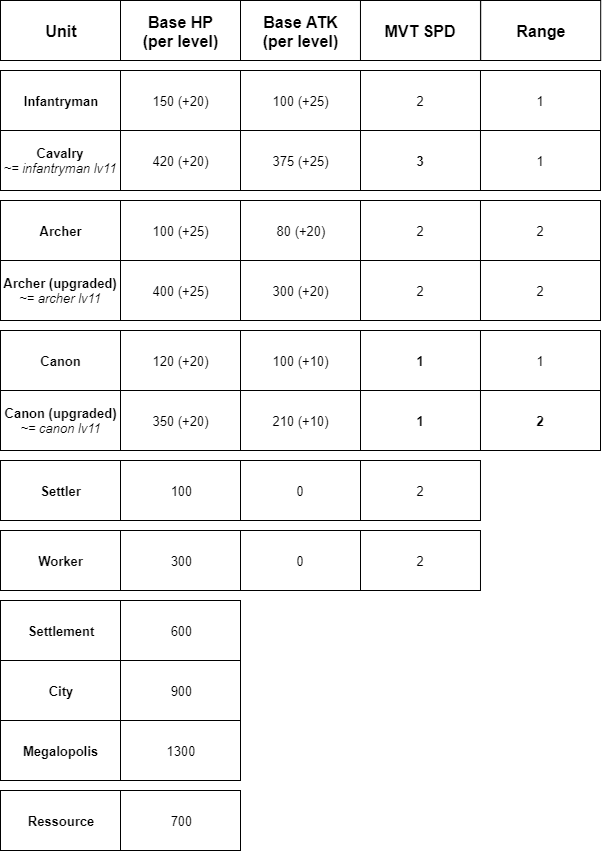
\includegraphics[width=0.9\textwidth]{units_stats}
    \caption{Statistiques par niveau}
\end{figure}
\begin{figure}[H]
    \centering
    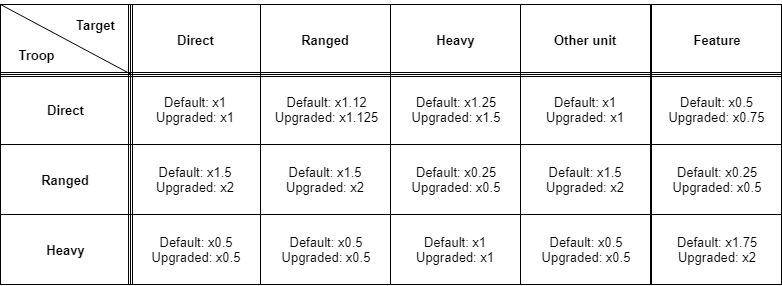
\includegraphics[width=0.9\textwidth]{damage_multipliers}
    \caption{Multiplicateurs de dégats en fonction des cibles}
\end{figure}

En somme, le gameplay est presque entièrement préparé, les différentes classes sont prévues et organisées, les attributs et méthodes sont listés, et il y a un début d’équilibrage. L'implémentation est désormais la priorité car il sera ensuite nécessaire d'ajuster les constantes pour équilibrer le jeu final.

\section{Assets (Cédric)}

Pour le design du jeu, nous avions pensé à un style un peu “cartoon” constitué de modèles 3D comportant peu de polygones. La principale raison étant que les objets sont ainsi plus facile à produire puisque tout est fait par nous-même via le logiciel \textit{Blender}. Le choix de \textit{Blender} était évident de par sa gratuité et parce que l’un des membres du groupe était déjà habitué à ce logiciel. Pour importer les modèles 3D de \textit{Blender} à \textit{Unity}, il a fallu les exporter en format FBX ce que \textit{Blender} peut faire facilement.

La ville d’un joueur évoluant au fil du temps suite à ses améliorations technologiques et à l’augmentation de sa population, il faut donc créer plusieurs modèles pour le même objet. Les unités sont elles aussi destinées à évoluer au fil des améliorations technologiques du joueur. Les unités et batiments auront une apparence inspirée de l'antiquité et/ou du moyen-âge. Chaque type d'unité offensive aura deux apparence, et les villes en auront trois, à chaque fois selon leur niveau/état (voir tableaux dans la partie Gameplay).

\newpage

La modélisation est chronophage, mais une fois les premiers modèles créés, les suivants peuvent les réutiliser et ainsi leur création est de plus en plus rapide.

Concernant les unités humaines, celles-ci se basent sur un modèle créé par nous-même et auront la même armature de base.

\begin{figure}[H]
    \centering
    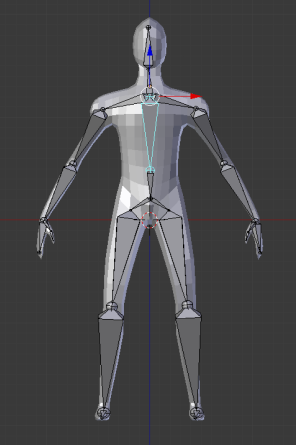
\includegraphics[width=0.3\textwidth]{unit_armature}
    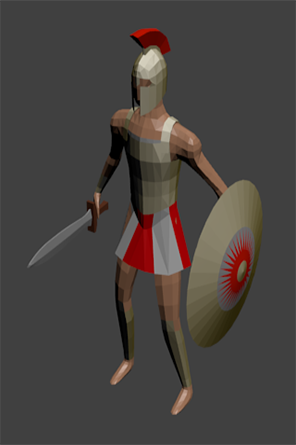
\includegraphics[width=0.3\textwidth]{swordmen}
    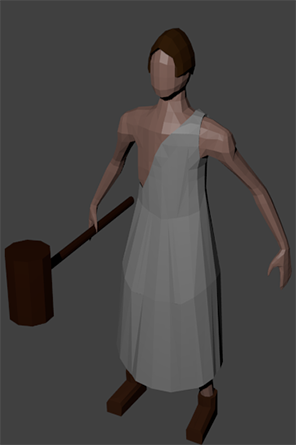
\includegraphics[width=0.3\textwidth]{worker}
    \caption{Unités et armature}
\end{figure}

La priorité a été mise sur les ressources de la carte et la ville, ainsi que sur les textures de la carte correspondant aux différents biomes. Celles-ci ont été faites grâce à un plugin de \textit{Unity} “NumberFlow” qui permet de générer des textures de manière procédurale.

\begin{figure}[H]
    \centering
    
\includegraphics[width=0.2\textwidth]{plain}
    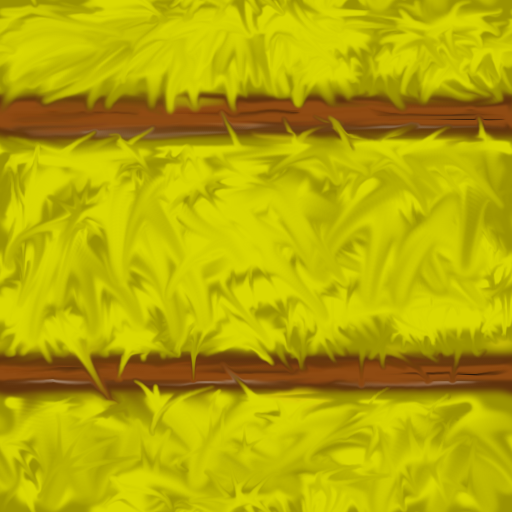
\includegraphics[width=0.2\textwidth]{straw_roof}
    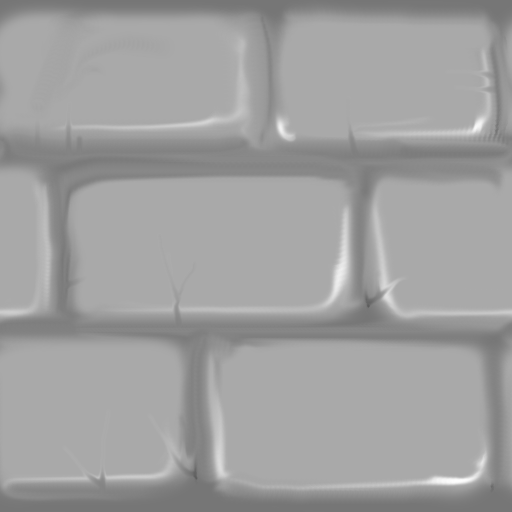
\includegraphics[width=0.2\textwidth]{wall}
    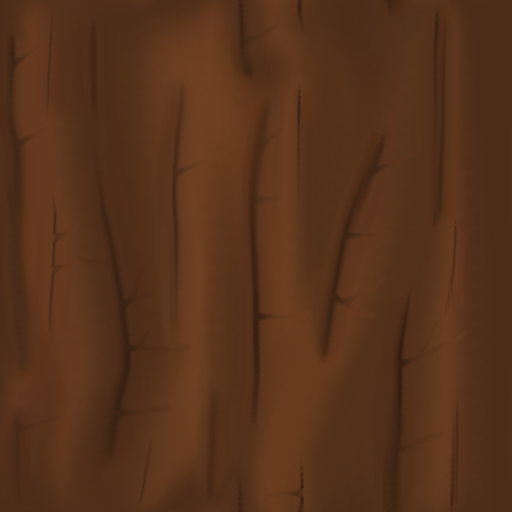
\includegraphics[width=0.2\textwidth]{wood}
    \caption{Textures}
\end{figure}

Les textures liées aux modèles 3D ont été faites mains grâce aux outils que proposaient \textit{Blender} et \textit{Krita}, un logiciel open-source de peinture numérique. Un bonus serait de pouvoir rajouter une \textit{Normal Map} pour donner des effets de relief et proposer ainsi un meilleur rendu.

\begin{figure}[H]
    \centering
    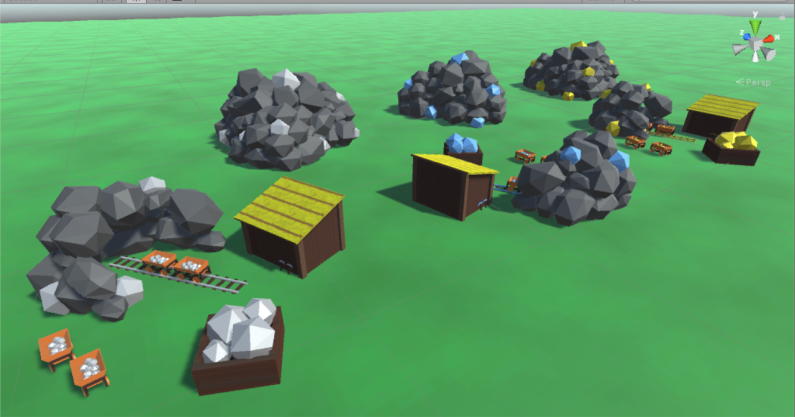
\includegraphics[scale=0.8]{mines}
    \caption{Exemple de feature: les mines}
\end{figure}

\section{Interface (Thibault \& Valérian)}

En ce qui concerne l’interface actuelle, il ne s’agit que d’une version créée dans le but de tester rapidement les fonctionnalités qui sont implémentées, faisant fi de l’esthétique. Cette interface test permet notamment à chaque membre de tester leur partie ainsi que de se rendre compte des besoins ergonomiques à prendre en compte dans la version finale.

Actuellement, le menu d’accueil est constitué uniquement de boutons, d’un slider pour sélectionner le nombre de joueurs, et de champs d’entrée textuelles servant à récupérer l’IP pour une connexion au serveur et le nom du joueur.

Du côté de l’interface de jeu, il s’agit de simples boutons permettant de sélectionner des options de modifications de la carte de jeu, ainsi qu’un menu d'accès à la sauvegarde et au chargement de différentes map.

\section{IA (Thibault)}

L’intelligence artificielle sera constituée de plusieurs fonctionnalités qui seront plus ou moins intense en fonction du niveau de difficulté choisi par le joueur :

\begin{itemize}[label=\textbullet]
	\item Des \textbf{tribus barbares} apparaîtront de manière régulière dans les alentours des villes, et pourront piller et attaquer les bâtiments et unités du joueur. Le niveau de technologie des unités barbares dépendra directement de celui du joueur ainsi que du niveau de difficulté.
	\item Des \textbf{malus} affectant directement l’économie interne du joueur pour ralentir le développement de son empire sur les différents aspects du jeu : économique, scientifique, et de production.
\end{itemize}

Les multiples niveaux de difficulté seront :

\begin{itemize}[label=\textbullet]
    \item \textbf{Facile :} des unités barbares d'un niveau faible par rapport au joueur (entre -3 et -2 niveaux de différence) qui apparaîtront de manière individuelle toutes les quinzaines de tours. Aucun malus sur l'empire.
    \item \textbf{Normal :} les barbares ont un niveau semblable ou légèrement plus fort que celui du joueur (entre 0 et +1 niveau de différence) et apparaissent par groupe de deux environ tous les 13 tours. Chaque aspect de développement de l'empire (économie, science, production) recevra un malus de -7.5\%.
    \item \textbf{Difficile :} des barbares féroces d'un niveau technologique plus élevé (+3 niveaux de différence) débarqueront par binômes environ tous les 10 tours. Le développement économique et de production reçoivent un malus de -12\%, tandis que celui scientifique de -9\%.
\end{itemize}

\section{Site Web (Valérian)}

En l’état actuel, le site possède un design basique permettant d’avoir une idée de son futur, ainsi qu’une page d’accueil fournissant des liens à tous les éléments nécessaires, que ce soit des logiciels utilisés, au jeu en lui-même, en passant par les rapports de soutenance. Il est hébergé grâce au service GitHub Pages.

\begin{figure}[H]
    \centering
    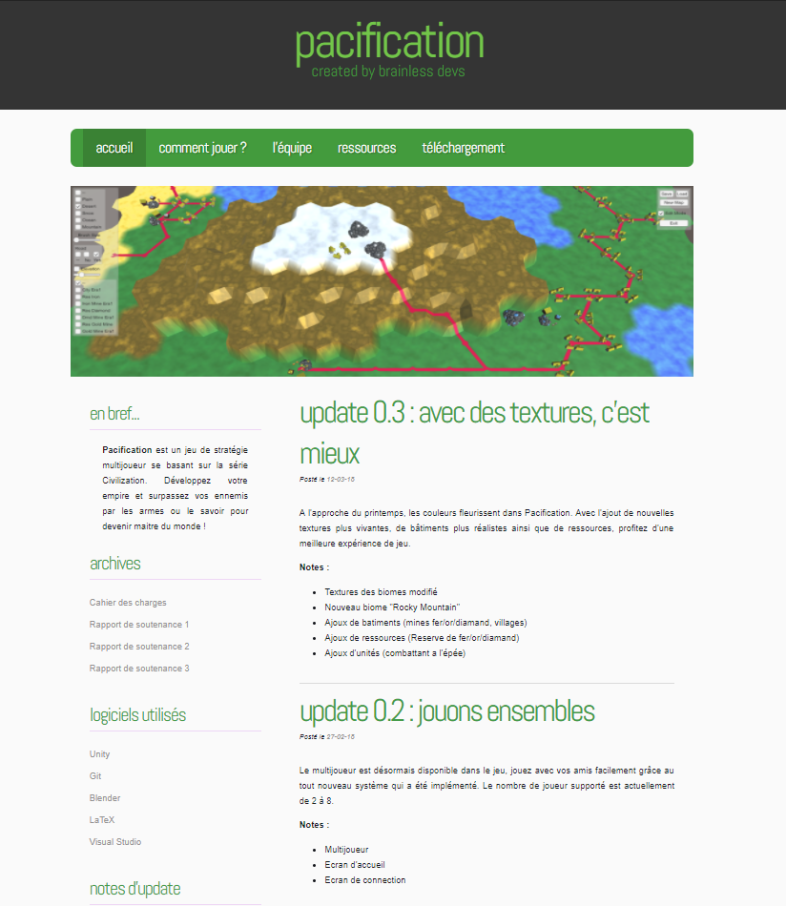
\includegraphics[scale=0.45]{homepage}
    \caption{Page d'accueil}
\end{figure}

\newpage

Un plan du site à été envisagé comme suit :

\begin{itemize}
\item Page d'accueil
\item Présentation du jeu
\item Comment jouer ?
    \begin{itemize}
    \item Solo
    \item Multijoueur
    \end{itemize}
\item Ressources utilisées
    \begin{itemize}
    \item Textures
    \item Sons
    \item Logiciels
    \item Autres assets
    \end{itemize}
\item Présentation de l'équipe
\item Notes de mises à jour
\item Téléchargements
    \begin{itemize}
    \item Cahier des charges
    \item Rapports de soutenances
    \item Jeu
    \end{itemize}
\end{itemize}

\chapter{Avances, retards, difficultés rencontrées}

\section*{Map}

Pas de retard à noter sur la map, le rendu visuel et l’implémentation sont satisfaisant. Toutes les caractéristiques fondamentales et nécessaires au développement du jeu sont désormais en place. La triangulation des hexagones n’a pas été une tâche facile, notamment pour mélanger les textures sur les cases voisines afin de ne pas avoir de transition brutale entre les biomes. Le système de route a de même pris du temps pour permettre de relier dans n’importe quelles directions des cases entre elles, et de réaliser l’affichage.

\section*{Multijoueur}

La progression du multijoueur suit les objectifs qui lui étaient fixés, c’est à dire d’établir une connexion entre les joueurs et de pouvoir transmettre des informations entre eux. Atteindre cet objectif n’a pas été simple car il a été nécessaire de se plonger dans un univers encore inconnu dans lequel nous n’avions aucune notion. Il a premièrement été envisagé d’utiliser la base multiplayer que propose \textit{Unity} toutefois nous nous sommes vite retrouvé coincé par des difficultés techniques concernant la synchronisation de la map dans le jeu. Réalisant que ces difficultés risquaient de poser problème plus tard dans le développement du jeu, nous avons opté pour une toute autre voie, construire notre propre système de serveur/clients. Appuyé par l’idée d’apprendre quelque chose de nouveau, il a fallu parcourir de nombreuses documentations et suivre plusieurs tutoriels sur le sujet pour parvenir à une base solide et fonctionnelle.

\section*{Gameplay}

Tout ce qui était prévu a été fait. J'aurais préféré commencer à implémenter des éléments afin d'obtenir quelque chose de concret dans le jeu, mais les shémas, tableaux et diagrammes me permettront de gagner beaucoup de temps lors de l'implémentation à venir. Le code ne sera pas bien compliqué, maintenant que tous les éléments sont prévus.

\section*{Assets}

La modélisation étant compliqué à faire et chronophage, le nombre d’asset créé n’est pas suffisant pour atteindre les 50\% voulus lors de la première soutenance. On se situerait plutôt à 40\%. Le processus de fabrication des assets devrait cependant être beaucoup plus rapide pour la suite.

\section*{Interface}

N’ayant pas établi d’objectifs visuels pour l’interface à ce niveau de développement, nous ne voulions qu’avoir des menus permettant de tester les fonctionnalités que nous implémentions. Cet objectif a été rempli.

\section*{Site web}

La construction du site web a pris de l'avance, ce qui permettra de passer davantage de temps sur d'autres tâches plus importantes.

\chapter{À venir}

\begin{itemize}
	\item \textbf{Map :} intégrer les unités, système de génération aléatoire de map.
	\item \textbf{Multijoueur :} transmission de la map, optimisation du processus d'échange de données.
	\item \textbf{Gameplay :} implémentation des classes, commencer à équilibrer l’économie interne.
	\item \textbf{Assets :} rajouter des assets, mettre en place des armatures sur les unités pour les animations, ajout d'effet visuel.
	\item \textbf{Interface :} menu principal clair, début d'interface de jeu, implémentation du changement de langue.
	\item \textbf{Site Web :} Compléter le site avec les pages manquantes.
\end{itemize}

\chapter{Expériences personnelles}

\begin{itemize}
	\item \textbf{Thibault :} L’implémentation de la map m’a permis d’apprendre concrètement à utiliser \textit{Unity}, et le fait de voir évoluer son propre jeu ainsi que les fonctionnalités qu’on développe rend cet apprentissage d’autant plus agréable et motivant pour la suite. Le fait que la map soit constituée d’hexagones a constitué un certain challenge pour le rendu visuel, la triangulation et le pavage.
    \item \textbf{Valérian :} Travailler sur ce projet pendant les mois qui ont précédé a été une expérience intéressante et instructive. J’ai pu découvrir comment manipuler certains outils tels que \textit{Git} et \textit{Unity}, mais ai aussi appris beaucoup concernant la programmation en général. Les parties dont j’ai pu m’occuper, notamment le réseau, m’ont permis d’apprendre des choses qui m'étaient totalement inconnues, et incité à chercher de la documentation plus poussée. J’ai aussi pu faire face à des problèmes qui m’ont beaucoup appris et grâce auxquels je retire une expérience nouvelle. J’ai trouvé particulièrement plaisant le fait de voir le projet se construire peu à peu, chaque semaine un peu plus complet.
	\item \textbf{Cédric :} Cette première période fut assez difficile pour ma part. Je m’étais pris à la création des asset 3D assez tard ce qui est une des raisons de mon retard sur ce qui était prévu. Néanmoins, je suis très heureux d’avoir pu utiliser les compétences que je possédais déjà sur \textit{Blender} car la modélisation et l’animation 3D sont des domaines que j’apprécie énormément. J’ai également appris de nouvelles techniques et suis devenu plus rapide sur mes créations. Je suis assez satisfait de ce que j’ai fait et je compte bien faire mieux plus tard. Le retard que j’ai pris m’aura au moins appris qu’il est essentiel de travailler sur le projet chaque semaine. D’autant plus que je dois également m’occuper de l’interface du jeu qui sera plus complexe que celle actuelle.
	\item \textbf{Antoine :} Période vraiment intéressante, qui m’a permis de réaliser à quel point faire un jeu (ou une application en général) relève d’abord d’une phase de réflexion importante pendant laquelle il faut planifier toutes les éventualités et les buts du projet. On voit le jeu prendre une direction, et on sait à quoi s’attendre dans les semaines qui viennent sans s’inquiéter de devoir ajouter/supprimer/modifier des bouts de code toutes les 5 minutes.
\end{itemize}

\chapter{Conclusion}

Cette première partie du projet s'achève donc sur un ressenti positif de notre part. La map et le multijoueur sont fonctionnels et posent les bases du jeu nécessaire à l'implémentation du gameplay. Les assets sources sont très satisfaisants malgrès le temps nécessaire à leur création. Le projet avance à un bon rythme, mais il reste encore beaucoup de travail à accomplir comme l'implémentation du gameplay, la génération de la map, l'optimisation du multijoueur et la création des assets restants.

Ce fût une première vraie expérience de groupe pour chacun, il a donc fallu apprendre à travailler à plusieurs que ce soit sur \textit{Git} d'un point de vue technique, mais aussi dans le développement d'une vision unique et cohérente du projet. Nous nous sommes réellement tous amusés à développer cette première partie du projet, qui, nous l'espérons, sera tout aussi plaisant à jouer.

\vfill

\begin{figure}[H]
    \centering
    
\includegraphics[width=0.8\textwidth]{project_real_mood}
\end{figure}

\end{document}
